% !TEX TS-program = pdflatex
% !TEX encoding = UTF-8 Unicode

% This is a simple template for a LaTeX document using the "article" class.
% See "book", "report", "letter" for other types of document.

\documentclass[11pt]{article} % use larger type; default would be 10pt

\usepackage[utf8]{inputenc} % set input encoding (not needed with XeLaTeX)

%%% Examples of Article customizations
% These packages are optional, depending whether you want the features they provide.
% See the LaTeX Companion or other references for full information.

%%% PAGE DIMENSIONS
\usepackage[a4paper, total={6in, 10in}]{geometry} % or letterpaper (US) or a5paper or....
% \geometry{margin=2in} % for example, change the margins to 2 inches all round
% \geometry{landscape} % set up the page for landscape
%   read geometry.pdf for detailed page layout information

\usepackage{graphicx} % support the \includegraphics command and options

% \usepackage[parfill]{parskip} % Activate to begin paragraphs with an empty line rather than an indent

%%% PACKAGES
\usepackage{booktabs} % for much better looking tables
\usepackage{array} % for better arrays (eg matrices) in maths
\usepackage{paralist} % very flexible & customisable lists (eg. enumerate/itemize, etc.)
\usepackage{verbatim} % adds environment for commenting out blocks of text & for better verbatim
\usepackage{subfig} % make it possible to include more than one captioned figure/table in a single float
% These packages are all incorporated in the memoir class to one degree or another...
\usepackage{listings}
\usepackage{xcolor}
\usepackage{amsmath}
\usepackage{float}

\definecolor{codegreen}{rgb}{0,0.6,0}
\definecolor{codegray}{rgb}{0.5,0.5,0.5}
\definecolor{codepurple}{rgb}{0.58,0,0.82}
\definecolor{backcolour}{rgb}{0.95,0.95,0.92}

\lstdefinestyle{mystyle}{
    backgroundcolor=\color{backcolour},   
    commentstyle=\color{codegreen},
    keywordstyle=\color{magenta},
    numberstyle=\tiny\color{codegray},
    stringstyle=\color{codepurple},
    basicstyle=\ttfamily\footnotesize,
    breakatwhitespace=false,         
    breaklines=true,                 
    captionpos=b,                    
    keepspaces=true,                 
    numbers=left,                    
    numbersep=5pt,                  
    showspaces=false,                
    showstringspaces=false,
    showtabs=false,                  
    tabsize=2
}

\lstset{style=mystyle}


%%% HEADERS & FOOTERS
\usepackage{fancyhdr} % This should be set AFTER setting up the page geometry
\pagestyle{fancy} % options: empty , plain , fancy
\renewcommand{\headrulewidth}{0pt} % customise the layout...
\lhead{}\chead{}\rhead{}
\lfoot{}\cfoot{\thepage}\rfoot{}

%%% SECTION TITLE APPEARANCE
\usepackage{sectsty}
\allsectionsfont{\sffamily\mdseries\upshape} % (See the fntguide.pdf for font help)
% (This matches ConTeXt defaults)

%%% ToC (table of contents) APPEARANCE
\usepackage[nottoc,notlof,notlot]{tocbibind} % Put the bibliography in the ToC
\usepackage[titles,subfigure]{tocloft} % Alter the style of the Table of Contents
\renewcommand{\cftsecfont}{\rmfamily\mdseries\upshape}
\renewcommand{\cftsecpagefont}{\rmfamily\mdseries\upshape} % No bold!

%%% END Article customizations

%%% The "real" document content comes below...

\title{AE 342 : Modeling and Analysis Lab, Session 5}
\author{Gaurav Gupta, SC21B026, Aerospace Engineering}
%\date{} % Activate to display a given date or no date (if empty),
         % otherwise the current date is printed 

\begin{document}
\maketitle

\section{Problem 1}
A simple 1D transient heat conduction is simulated. The governing equations andboundary conditions are provided as follows.


\begin{equation}
\frac{du}{dt} = \frac{d^2u}{dx^2}, \text{ }0 < x < 1, \text{ }t>0
\end{equation}

\begin{equation}
u(x=0) = x-x^2 \text{,  } u(0,t) = u(1,t)=0 
\end{equation}

The problem is solved in FreeFEM++ using the given code for a 1D domain. 

\begin{figure}[H]
\centering
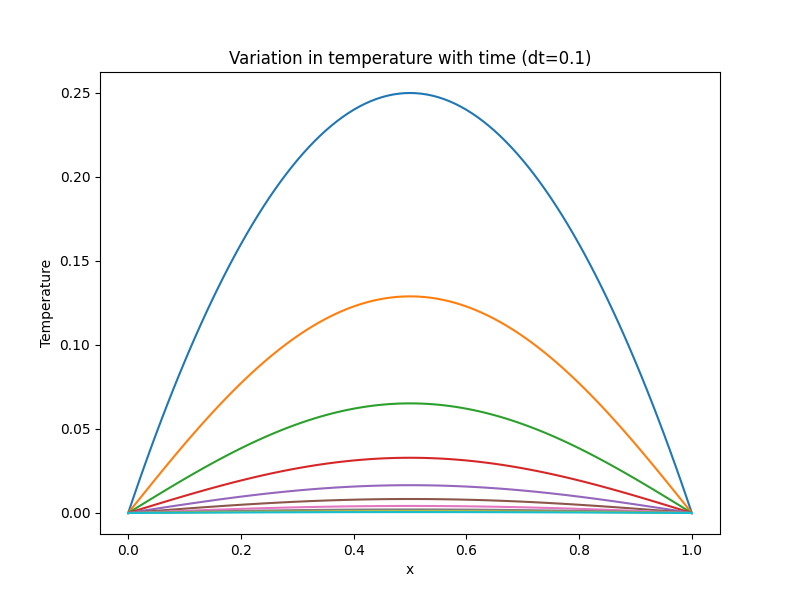
\includegraphics[width=0.95\textwidth]{figures/p111.png}
\caption{FreeFEM transient solution of the problem. As the time progresses the temperature across the whole domain reaches 0.}
\end{figure}
\newpage
\begin{lstlisting}[language=C++, caption=Problem 1 Code ]
load "msh3"
real m = 100;
int l=1;
real dt = 0.001;
real T = 1;
meshL Th = segment(m,[x*l]);
func T0 = x - x^2; 

ofstream ff("result1.csv");

fespace Vh(Th, P1);
Vh t=T0, v, told;

problem heateqn(t,v)= int1d(Th)(dx(t)*dx(v))
				+int1d(Th)(v*t/dt)
				-int1d(Th)(v*told/dt)
				+on(1,2, t=0); //comment the boundary condition to apply the neumann b.c. erquired in the section 1.2

//ff<<"t"<<",";
for(int j=0; j<=m; j++){
		if(j==m){
			ff <<"x"<<j;
		}else{
			ff <<"x"<<j<<",";
		}
	}
ff<<endl;
for(real i=0; i<=T; i+=dt){
	told = t;
	heateqn;
	//ff<<"t"<<i/dt<<",";
	for(int j=0; j<=m; j++){
		if(j==m){
			ff <<told[][j];
		}else{
			ff <<told[][j]<<",";
		}
	}
	ff<<endl;
}

//plot(t, wait=true, value=true);
\end{lstlisting}
\vspace{0.5cm}
\subsection{Comparision with Analytical Solution}
The analytical solution for the problem is given as,
\begin{equation}
u(x,t) = \frac{4}{\pi^3}\sum_{n=1}^{\infty}\frac{1 - (-1)^n}{n^3}e^{-n^2\pi^2 t}sin(n\pi x)
\end{equation}
 The solution of FreeFEM is compared to the analytical solution at time $t=0.2s$,
\begin{figure}[H]
\centering
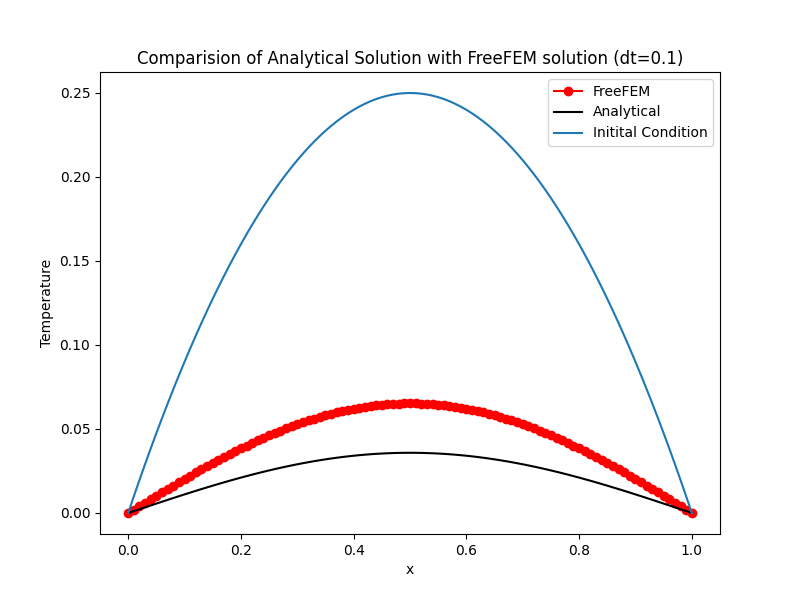
\includegraphics[width=0.85\textwidth]{figures/p121.png}
\caption{Comparision of the FreeFEM Solution with analytical solution for Problem 1.}
\end{figure}

\subsection{Neumann Boundary Conditions}
In the current problem, both the ends are insulated instead of the Dirchlet boundary condition of $U=0$. This gives the solution of the problem in FreeFEM as,

\begin{figure}[H]
\centering
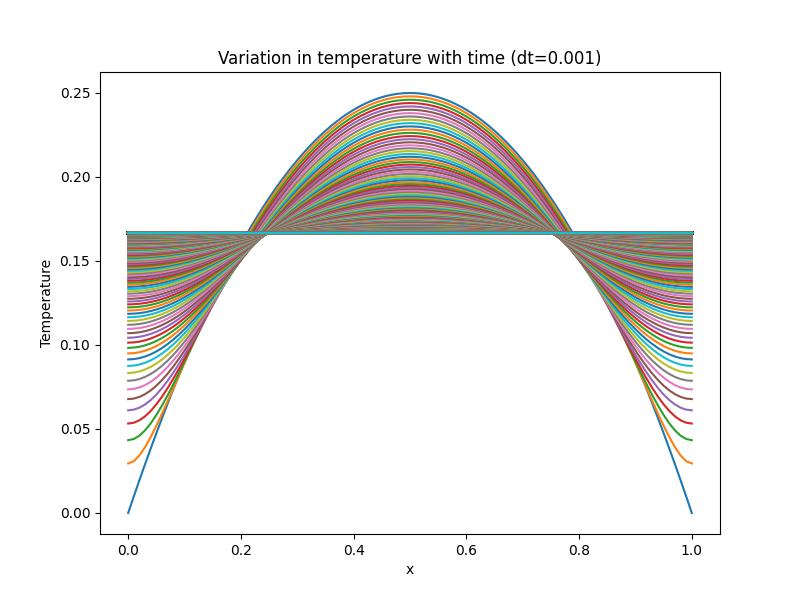
\includegraphics[width=0.85\textwidth]{figures/p11001n.png}
\caption{FreeFEM transient solution of the problem. As the time progresses the temperature across the whole domain reaches a constant temperature.}
\end{figure}

\subsection{Time Convergence Study}
The time step $(dt)$ used to solve the problem is varied between 0.1, 0.01 and 0.001 while keeping the grid size $(dx=0.01)$ constant. As we reduce $dt$, the error in the FreeFEM solution reduces significantly as compared to the analytical solution.

\begin{figure}[H]
\centering
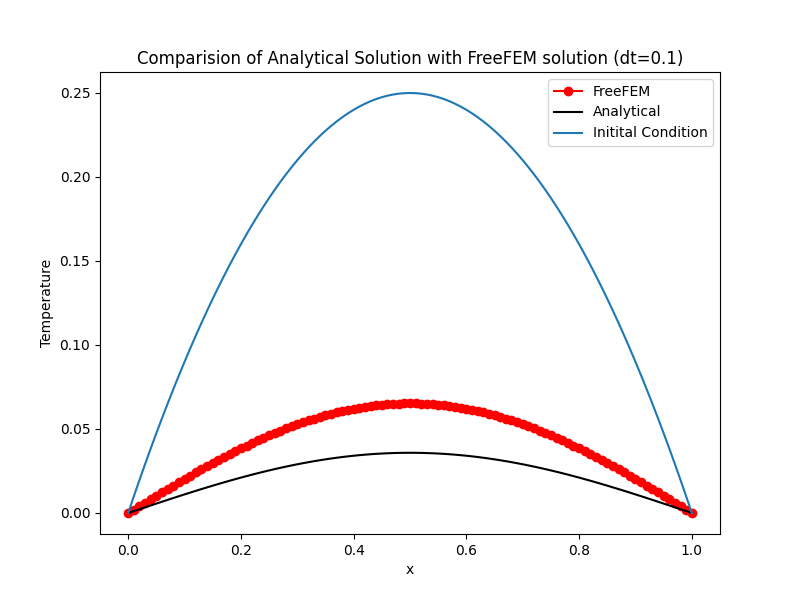
\includegraphics[width=0.35\textwidth]{figures/p121.png}
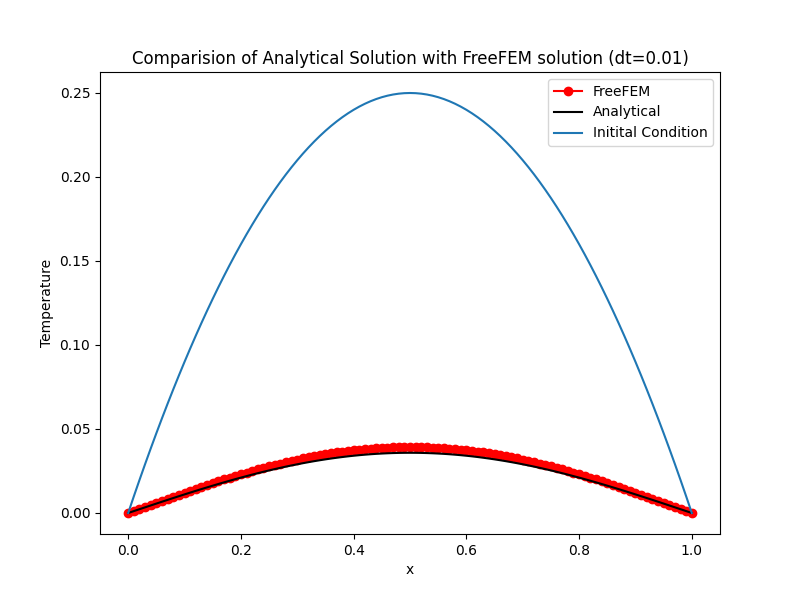
\includegraphics[width=0.35\textwidth]{figures/p1201.png}
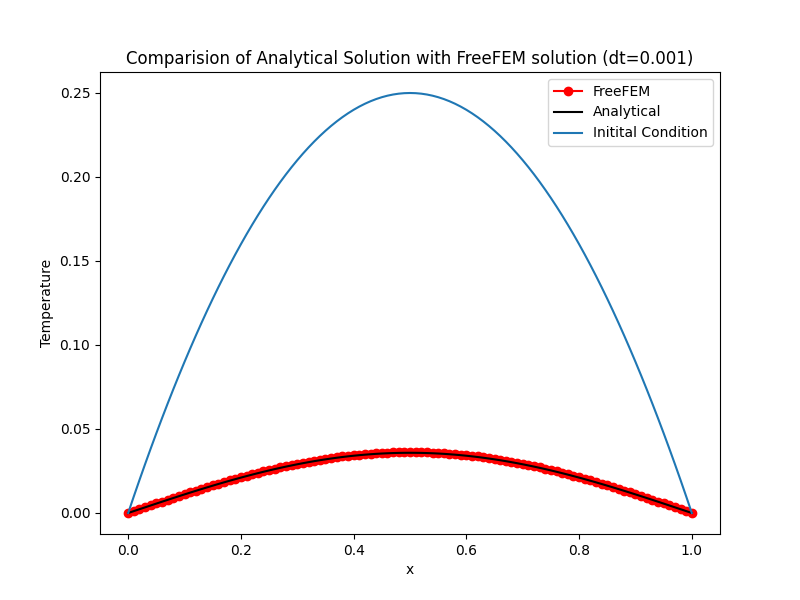
\includegraphics[width=0.35\textwidth]{figures/p12001.png}
\caption{Time step convergence study of FreeFEM Solution for Problem 1.}
\end{figure}

\subsection{Grid Convergence Study}
The grid size $(dx)$ used to solve the problem is varied between 0.1, 0.01 and 0.001 while keeping the time step $(dt=0.001)$ constant. No significant change in the error in the FreeFEM solution was observed for the tested grid size as compared to the analytical solution.

\begin{figure}[H]
\centering
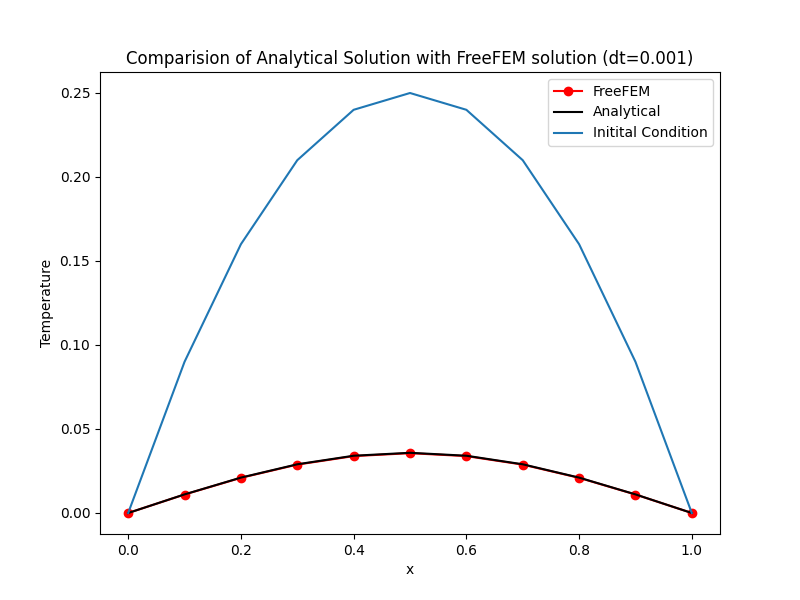
\includegraphics[width=0.35\textwidth]{figures/p12001x1.png}
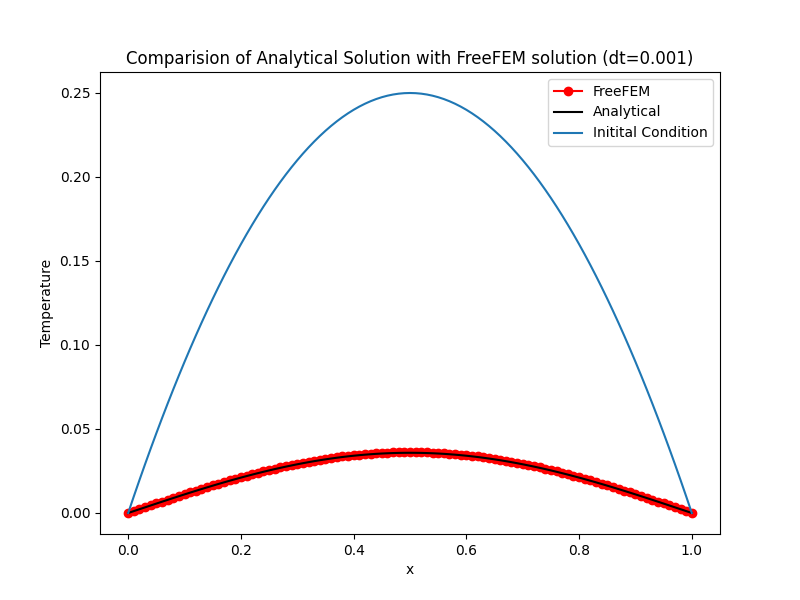
\includegraphics[width=0.35\textwidth]{figures/p12001.png}
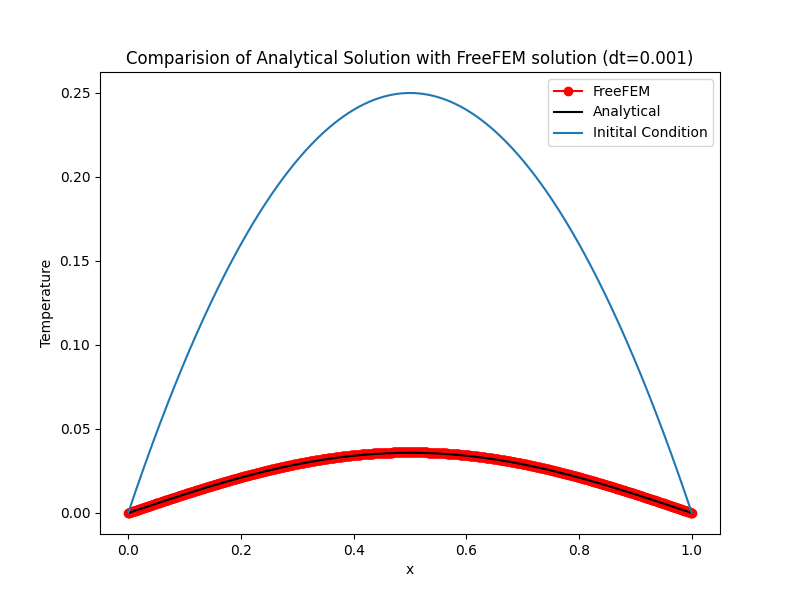
\includegraphics[width=0.35\textwidth]{figures/p12001x001.png}
\caption{Time step convergence study of FreeFEM Solution for Problem 1.}
\end{figure}
\newpage
\section{Problem 2}
A combination of Dirichlet and Neumann boundary condition is considered for this problem. The governing equation, boundary conditions, and initial conditions are stated below
\begin{equation}
u_t = u_{xx}
\end{equation}
\begin{center}
for $0<x<2$, $t>0$
\end{center}
\begin{equation}
u(0,x) = 
\begin{cases}
x & x\leq 1\\
2-x & 1<x\leq 2
\end{cases}
\end{equation}

\begin{center}
$u(0,t) = u_x(2,t) = 0$
\end{center}

\vspace{0.5cm}

The problem is solved in FreeFEM++ using the given code for a 1D domain. 

\begin{figure}[H]
\centering
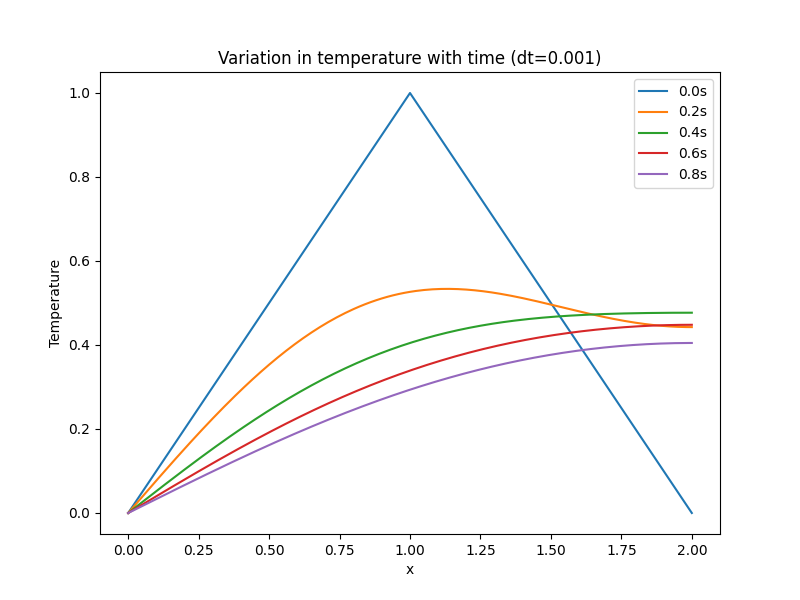
\includegraphics[width=\textwidth]{figures/p21.png}
\caption{FreeFEM transient solution of the problem. As the time passes the temperature at the right boundary with insulation b.c. increases until it reaches steady state.}
\end{figure}
\newpage
\begin{lstlisting}[language=C++, caption=Problem 2 Code ]
load "msh3"
real m = 200;
int l=2;
real dt = 0.001;
real T = 1;
meshL Th = segment(m,[x*l]);
func real T0(){
	if(x<=1){
		return x;
	}else{
		return 2-x;
	}
} 


ofstream ff("result2.csv");

fespace Vh(Th, P1);
Vh t=T0(), v, told;

problem heateqn(t,v)= int1d(Th)(dx(t)*dx(v))
				+int1d(Th)(v*t/dt)
				-int1d(Th)(v*told/dt)
				+on(1, t=0);


//ff<<"t"<<",";
for(int j=0; j<=m; j++){
		if(j==m){
			ff <<"x"<<j;
		}else{
			ff <<"x"<<j<<",";
		}
	}
ff<<endl;
for(real i=0; i<=T; i+=dt){
	told = t;
	heateqn;
	//ff<<"t"<<i/dt<<",";
	for(int j=0; j<=m; j++){
		if(j==m){
			ff <<told[][j];
		}else{
			ff <<told[][j]<<",";
		}
	}
	ff<<endl;
}

//plot(t, wait=true, value=true);
\end{lstlisting}
\newpage
\subsection{Comparision with Analytical Solution}
The analytical solution for the problem is given as,
\begin{equation}
u(x,t) = \frac{32}{\pi^3}\sum_{n=1}^{\infty}sin\left(\frac{(2n - 1)\pi}{4}\right)\frac{1 - cos\left(\frac{(2n - 1)\pi}{4}\right)}{(2n - 1)^2}e^{\frac{(2n-1)^2}{16}\pi^2 t}sin\left(\frac{(2n - 1)\pi}{4} x\right)
\end{equation}
 The solution of FreeFEM is compared to the analytical solution at time $t=0.2s$,
\begin{figure}[H]
\centering
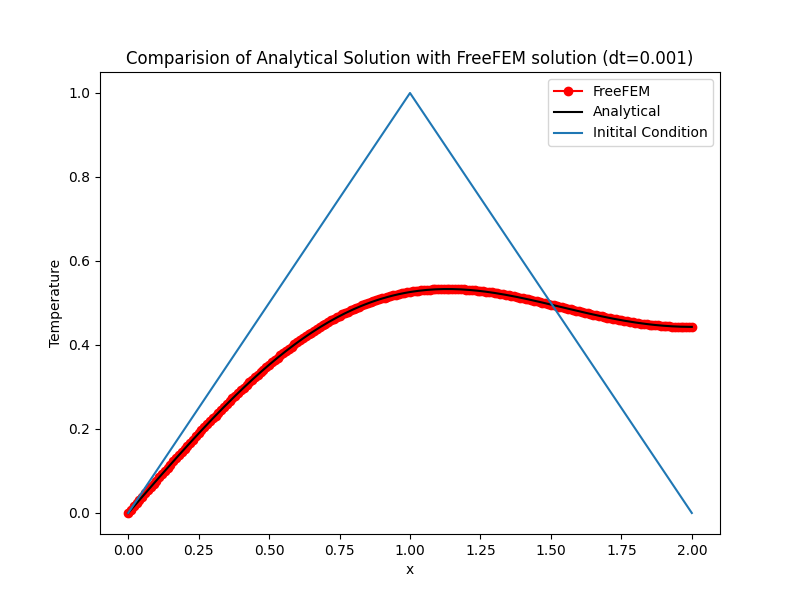
\includegraphics[width=\textwidth]{figures/p22.png}
\caption{Comparision of the FreeFEM Solution with analytical solution for Problem 2.}
\end{figure}
\newpage
\section{Problem 3}
In practical problems, there can be instances when we encounter non-standard or non-homogeneous boundaries. Here, a non-homogeneous boundary condition problem is discussed,

\begin{equation}
\frac{du}{dt} = \frac{d^2u}{dx^2}, \text{ }0 < x < 3, \text{ }t>0
\end{equation}

\begin{equation}
u(x=0) = 4x-x^2 \text{,  } u(0,t) =0\text{, } u(3,t)=3 
\end{equation}

\vspace{0.5cm}

The problem is solved in FreeFEM++ using the given code for a 1D domain. 

\begin{figure}[H]
\centering
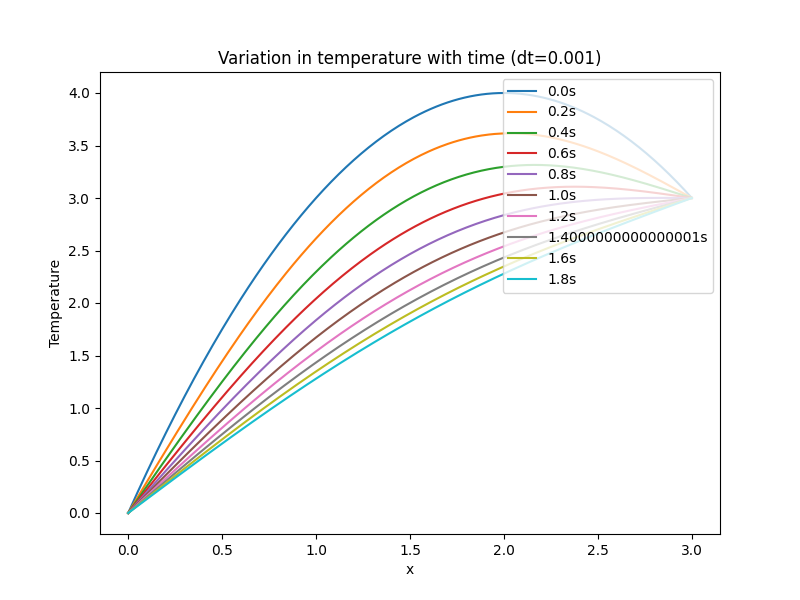
\includegraphics[width=\textwidth]{figures/p31.png}
\caption{FreeFEM transient solution of the problem. As the time passes the temperature distribution in the domain linearizes and a linear distribution exists at steady state.}
\end{figure}
\newpage
\begin{lstlisting}[language=C++, caption=Problem 3 Code ]
load "msh3"
real m = 300;
int l=3;
real dt = 0.001;
real T = 2;
meshL Th = segment(m,[x*l]);
func T0 = 4*x - x^2; 

ofstream ff("result3.csv");

fespace Vh(Th, P1);
Vh t=T0, v, told;

problem heateqn(t,v)= int1d(Th)(dx(t)*dx(v))
				+int1d(Th)(v*t/dt)
				-int1d(Th)(v*told/dt)
				+on(1, t=0)
				+on(2, t=3);


//ff<<"t"<<",";
for(int j=0; j<=m; j++){
		if(j==m){
			ff <<"x"<<j;
		}else{
			ff <<"x"<<j<<",";
		}
	}
ff<<endl;
for(real i=0; i<=T; i+=dt){
	told = t;
	heateqn;
	//ff<<"t"<<i/dt<<",";
	for(int j=0; j<=m; j++){
		if(j==m){
			ff <<told[][j];
		}else{
			ff <<told[][j]<<",";
		}
	}
	ff<<endl;
}

//plot(t, wait=true, value=true);
\end{lstlisting}

\subsection{Comparision with Analytical Solution}
The analytical solution for the problem is given as,
\begin{equation}
u(x,t) = \frac{32}{\pi^3}\sum_{n=1}^{\infty}sin\left(\frac{(2n - 1)\pi}{4}\right)\frac{1 - cos\left(\frac{(2n - 1)\pi}{4}\right)}{(2n - 1)^2}e^{\frac{(2n-1)^2}{16}\pi^2 t}sin\left(\frac{(2n - 1)\pi}{4} x\right)
\end{equation}
 The solution of FreeFEM is compared to the analytical solution at different times,
\begin{figure}[H]
\centering
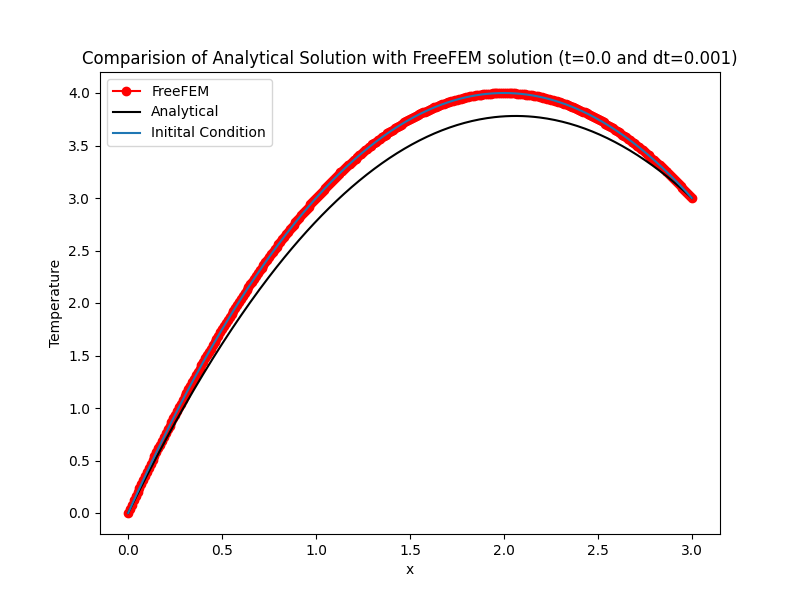
\includegraphics[width=0.48\textwidth]{figures/p320.png}
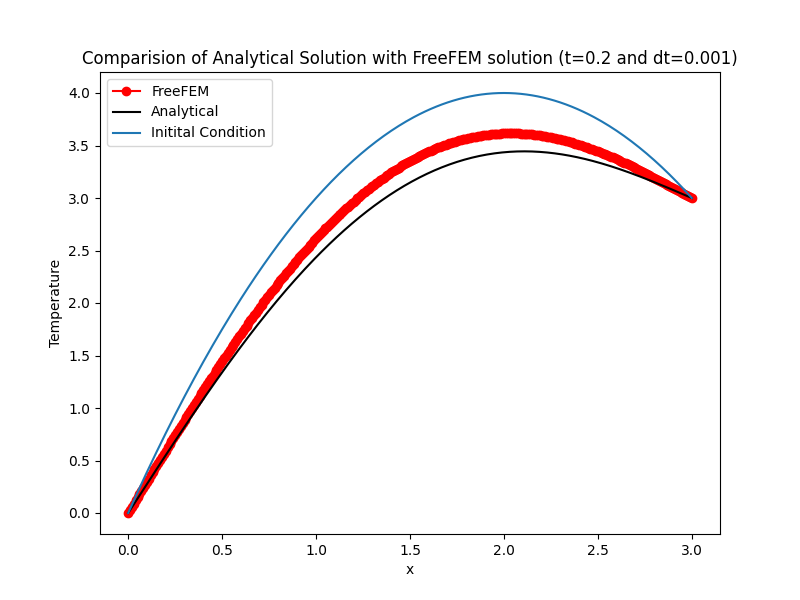
\includegraphics[width=0.48\textwidth]{figures/p321.png}
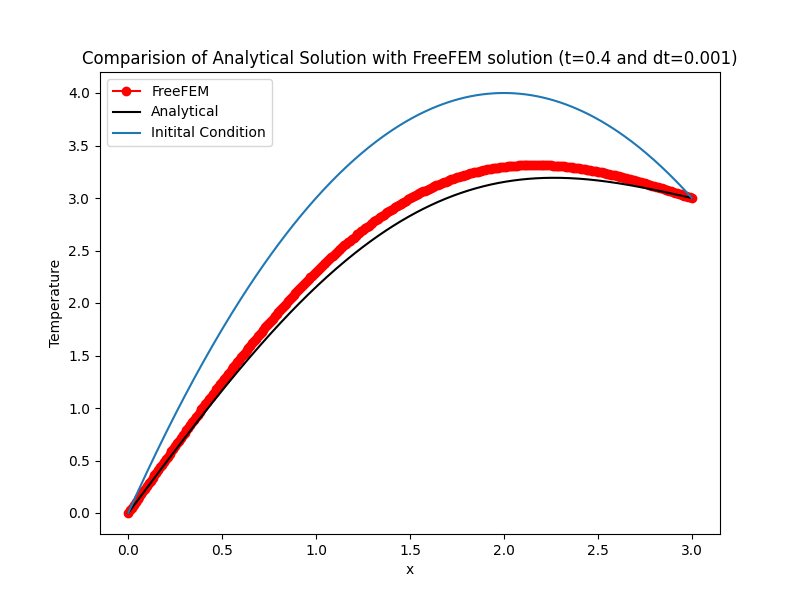
\includegraphics[width=0.48\textwidth]{figures/p322.png}
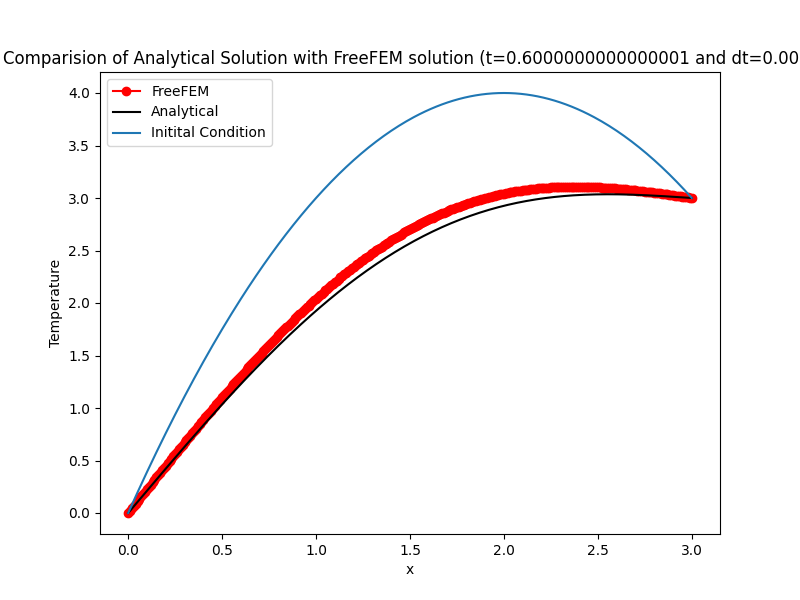
\includegraphics[width=0.48\textwidth]{figures/p323.png}
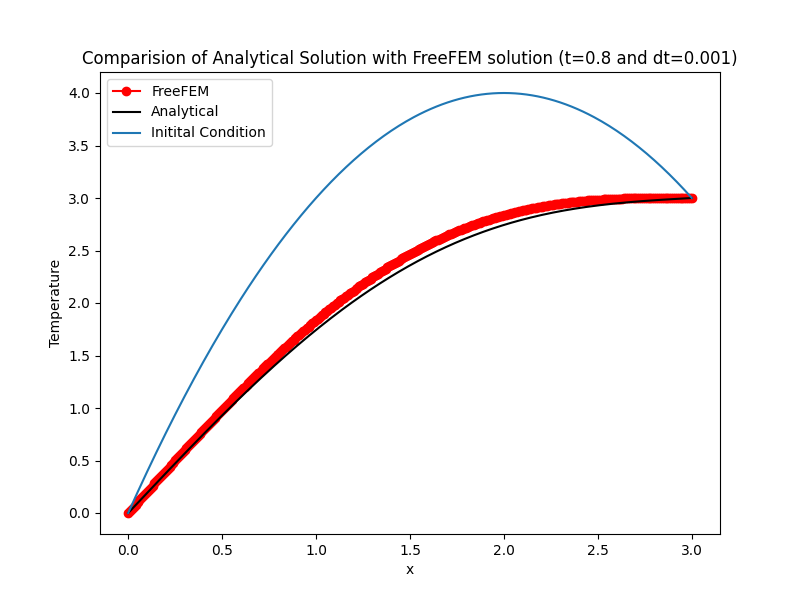
\includegraphics[width=0.48\textwidth]{figures/p324.png}
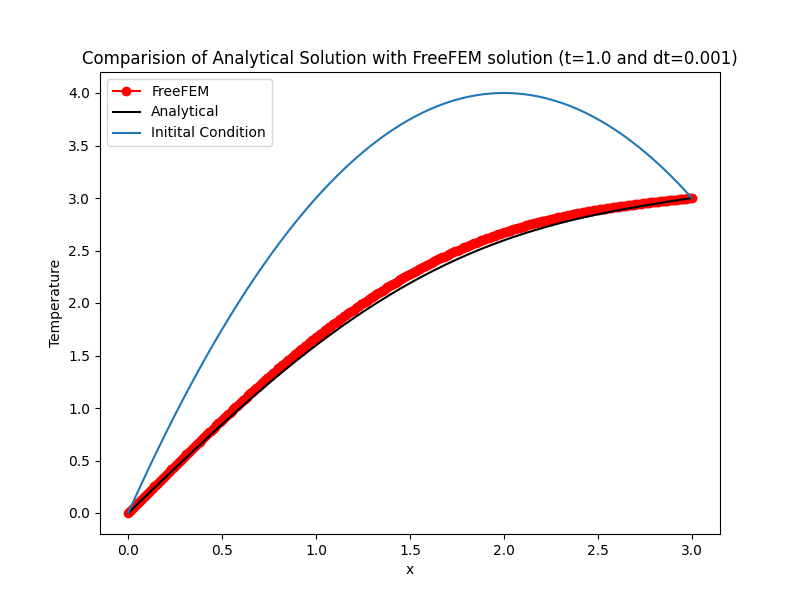
\includegraphics[width=0.48\textwidth]{figures/p325.png}
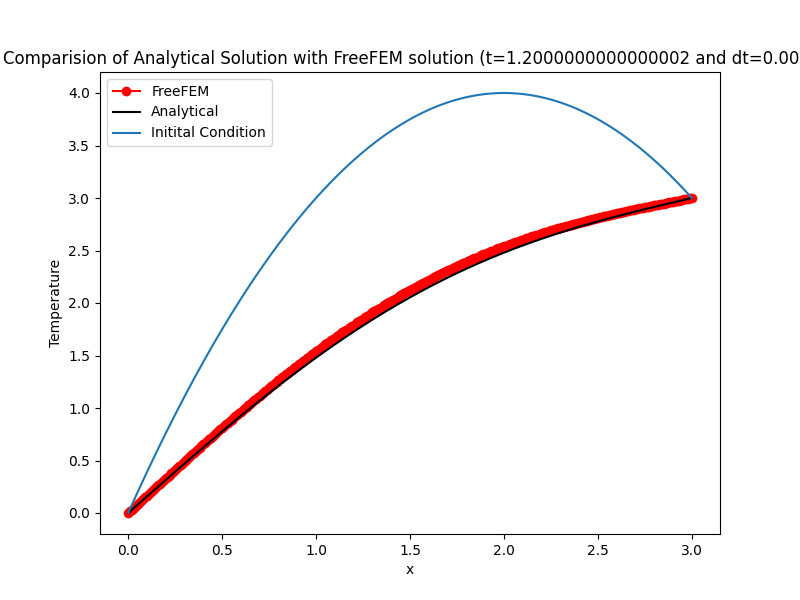
\includegraphics[width=0.48\textwidth]{figures/p326.png}
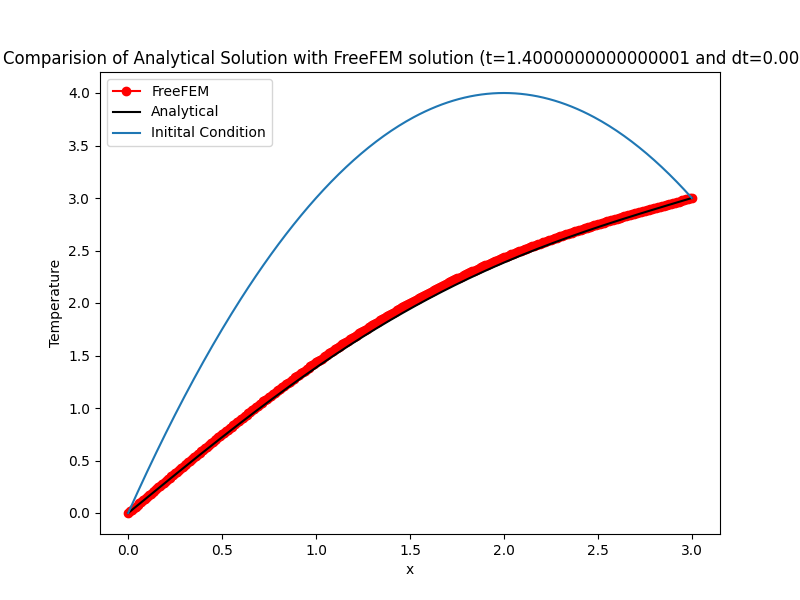
\includegraphics[width=0.48\textwidth]{figures/p327.png}
\caption{Comparision of the FreeFEM Solution with analytical solution for Problem 3. The error in the FreeFEM solution reduces as time passes and reaches steady state as compared to the analytical solution.}
\end{figure}
\newpage
\section{Problem 4}
A problem similar to the previous one attempted. However in this problem a neumann condition of a constant gradient is given at the left boundary. The governing equations initial conditions and the boundary conditions are summarised below.

\begin{equation}
\frac{du}{dt} = \frac{d^2u}{dx^2}, \text{ }0 < x < 1, \text{ }t>0
\end{equation}

\begin{equation}
u(x=0) = 0 \text{,  } u_x(0,t) =-1\text{, } u_x(1,t)=0 
\end{equation}

\vspace{0.5cm}

The problem is solved in FreeFEM++ using the given code in a 2D domain. 

\begin{figure}[H]
\centering
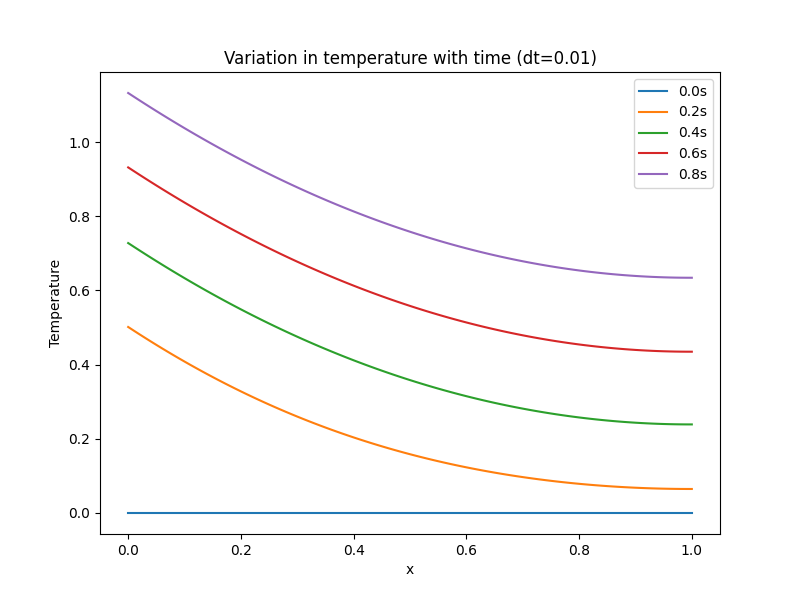
\includegraphics[width=\textwidth]{figures/p41.png}
\caption{FreeFEM transient solution of the problem. As the time passes the temperature distribution in the domain increases throughout the domain.}
\end{figure}
\newpage
\begin{lstlisting}[language=C++, caption=Problem 4 Code ]
load "msh3"
real m = 100;
int l=1;
real dt = 0.01;
real T = 2;
mesh Th = square(m,m,[x*l, y*l]);
real T0 = 0; 

ofstream ff("result4.csv");

fespace Vh(Th, P1);
Vh t=T0, v, told;

problem heateqn(t,v)= int2d(Th)(dx(t)*dx(v))
				+int2d(Th)(v*t/dt)
				-int2d(Th)(v*told/dt)
				+int1d(Th,4)(v*(-1));


//ff<<"t"<<",";
for(int j=0; j<=m; j++){
		if(j==m){
			ff <<"x"<<j;
		}else{
			ff <<"x"<<j<<",";
		}
	}
ff<<endl;
for(real i=0; i<=T; i+=dt){
	told = t;
	heateqn;
	//ff<<"t"<<i/dt<<",";
	for(int j=0; j<=m; j++){
		if(j==m){
			ff <<told[][j];
		}else{
			ff <<told[][j]<<",";
		}
	}
	ff<<endl;
}

//plot(t, wait=true, value=true);
\end{lstlisting}

\subsection{Comparision with Analytical Solution}
The analytical solution for the problem is given as,
\begin{equation}
u(x,t) = \frac{1}{2} (x^2 + 2t) - x + \frac{1}{3} - \frac{2}{\pi^2}\sum_{n=1}^{\infty} \frac{1}{n^2} e^{-n^2 \pi^2 t} cos(n\pi x)
\end{equation}
 The solution of FreeFEM is compared to the analytical solution at different times,
\begin{figure}[H]
\centering
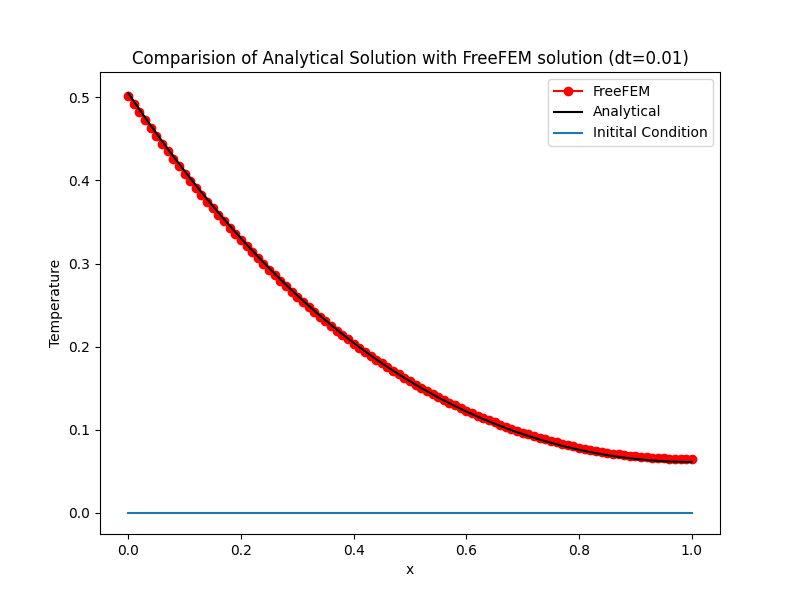
\includegraphics[width=0.9\textwidth]{figures/p42.png}
\caption{Comparision of the FreeFEM Solution with analytical solution for Problem 4.}


\includegraphics[width=0.9\textwidth]{figures/p411.png}
\caption{FreeFEM transient solution of the problem at time t=0.18s}
\end{figure}
\end{document}

